\documentclass[10pt,journal,a4paper]{IEEEtran}
\usepackage{tikz}
\usepackage{amsmath}
\usepackage{amssymb}
\usepackage{graphicx}
\usepackage{caption}
\usepackage{cleveref}
\usepackage{subcaption}

\begin{document}
%
% paper title
% can use linebreaks \\ within to get better formatting as desired
\title{Report for the NOOC project}
\author{Ismail Bouanani and Jean-Baptiste Cordonnier}

\IEEEcompsoctitleabstractindextext{
\begin{abstract}
Rumor spreading is a well known problem with multiple applications, from information broadcast in complex distributed systems to analysis of viral content on social networks. This project report will go over the paper of Guo and Sun \cite{guosun}. We aim at providing a good understanding of the concept and the mathematical tool used to show the $O(\log n)$ bound for the time steps needed to spread a rumor. We will then provide simulation of this algorithm on specific graphs. Finally we will explain the number of bits of randomness needed to run the algorithm.
\end{abstract}
}

\newcommand{\norm}[1]{\left\lVert#1\right\rVert}
\newtheorem{theorem}{Theorem}
\newtheorem{definition}{Definition}
\renewcommand{\l}{\left}
\renewcommand{\r}{\right}
\renewcommand{\P}[1]{\mathbf{P}\l\{#1\r\}}
\newcommand{\E}[1]{\mathbf{E}\l[#1\r]}

% make the title area
\maketitle
\IEEEdisplaynotcompsoctitleabstractindextext

\section{Introduction}

\begin{theorem}[Main result]
  Let $G$ be a graph with $n$ nodes, spectral gap $\alpha$ and irregularity $\beta$. Then there is an explicit protocol using $O(C' \log n) + \tilde O(\log n)$ random bits sucht that with high probability all nodes get the rumor in $T=O(C \log n)$ rounds, where $C = (1/\alpha) \cdot \beta^2 \max(1, 1/(\alpha \cdot \Delta ^ {0.499}))$
\end{theorem}

\section{Rumor spreading protocol}

The rumor spreading protocol is the simplest algorithm we can come with in order to solve the rumor spreading problem. Given a starting node $n_0$ (the source of the gossip), we keep track of a set of informed nodes $S = \{n_0\}$. At each time step of the algorithm, each informed node will select randomly (uniformly to simplify) one of his neighbor and inform him. Step after step the informed nodes set will grow until it contains all the vertex of $G$. Once a node is informed he becomes an informer and will spread the gossip at all the following time steps.

\section{Markov chains set-up}

The analysis in the paper of Guo and Sun \cite{guosun} compares the problem of gossip spreading to many random walks in parallel. Whenever a node $u$ pushes the information to an uninformed node $v$, one random walk stays in $u$ and another one goes to $v$. The random walk that "stays" in the same node is called $lazy$ while the other one is non-lazy (or $\overline{lazy}$). This split of random walks represents the fact that the information is now in $u$ and in $v$, $u$ will continue to spread this knowledge in the following rounds.

\begin{figure}[h]
\centering
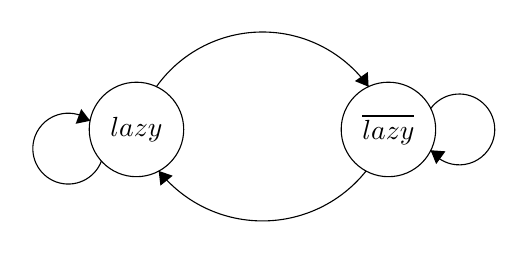
\begin{tikzpicture}[scale=0.2]
\tikzstyle{every node}+=[inner sep=0pt]
\draw [black] (26.1,-26.6) circle (3);
\draw (26.1,-26.6) node {$lazy$};
\draw [black] (42.1,-26.6) circle (3);
\draw (42.1,-26.6) node {$\overline{lazy}$};
\draw [black] (40.688,-29.229) arc (-38.4609:-141.5391:8.413);
\fill [black] (27.51,-29.23) -- (27.62,-30.17) -- (28.4,-29.54);
\draw [black] (27.358,-23.895) arc (144.65362:35.34638:8.265);
\fill [black] (40.84,-23.89) -- (40.79,-22.95) -- (39.97,-23.53);
\draw [black] (23.878,-28.598) arc (-20.31276:-308.31276:2.25);
\fill [black] (23.16,-26.05) -- (22.59,-25.3) -- (22.24,-26.24);
\draw [black] (44.78,-25.277) arc (144:-144:2.25);
\fill [black] (44.78,-27.92) -- (45.13,-28.8) -- (45.72,-27.99);
\end{tikzpicture}
\caption{Random walk state}
\label{fig:lazyFSM}
\end{figure}

We define two types of random walks when the information is spread through the graph: the forward and the backward random walks. Forward random walks start from the source $s$ while backward random walks are used only in the analysis and start from a targeted node $t$. In fact if a node $u$ pushes information to a node $v$, we can also say that $v$ "pulls" the information from $u$ and there exists a random walk called reverse having a step from $v$ to $u$, that remains true if and only if $u$ the only node that pushed to $v$ is $u$.Then to know if a node $t$ has been informed, we only need to show that there exists a node $v$ reached by a forward random walk from $s$ and by a backward random walk from $t$.

We can consider all the random walks pattern after $k$ steps as $S \in \mathcal C_k = \{ lazy, \overline{lazy} \}^k$. We define the indicator random variable $X_{u,v}^S$ (resp. $Y_{u,v}^S$) that the forward (resp. backward) random walk with pattern $S$ and initial node $u$ will end up at node $v$. To show that a node $w$ is reached by the gossip in $T$ steps we need to find a vertex $u$ such that $X_{s,u}^{S}Y_{w,u}^{S'} = 1$ with $|S| = |S'| = T/2$. We can now lower bound the probability of a node to be informed in $T$ steps as follow

\begin{align*}
  \P{w \text{ informed in $T$ rounds}} \geq \P{\sum_{S,S'\in \mathcal C_k, u\in V[G]} X_{s,u}^S Y_{w,u}^{S'} > 0}
\end{align*}

In the next section we will analyze this lower bound thanks to random walks taken individually and pair wisely.

\section{Bound analysis}

The need to analyze two random walks together to get a lower bound of the expectation leads us to use Markov chain coupling. Formally, a matrix coupling is defined as follow:

\begin{definition}
  A stochastic matrix $\mathbf{M'' \in \mathbb{R}^{n\times n} \otimes \mathbb{R}^{n\times n}}$ is a coupling of $\mathbf{M,M''} \in \mathbb{R}^{n\times n}$ if $\sum_{x\in[n]} \mathbf{M''}_{(u,w)(v,x)} = \mathbf{M}_{u,v}$ for any $u,w,v \in [n]$ and $\sum_{v\in[n]} \mathbf{M''}_{(u,w)(v,x)} = \mathbf{M'}_{w,x}$.
\end{definition}

The intuition behind this is that we are mixing two Markov chains together and coupling their state. Now the state of $\mathbf{M''}$ will contain the state of both matrices, and the two matrices will behave independently according to their own transitions distributions. The paper \cite{guosun} also defines lazy Markov chain with a slack parameter $\gamma$ that represents the probability for a Markov chain to stay idle in the same state (by increasing the diagonal probabilities):

\[
  \mathcal L _ \gamma (\mathbf{M}) \triangleq (1-\gamma) \mathbf{I} + \gamma \mathbf{M}
\]

Finally, we define a lazy coupling of $\mathbf{M}$ and $\mathbf{M'}$ noted $\mathcal L_{\gamma, \gamma'}(\mathbf{M''})$ to be the coupling of $\mathcal L_\gamma(\mathbf{M})$ and $\mathcal L_{\gamma'}(\mathbf{M'})$. The last tool needed to characterize our bound with Markov chain is the Doeblin coupling \cite{coupling}. It reflects the fact that when two random walks are in the same state $u$ at the same time step $t$, they will stay together for all the remaining steps because the node $u$ can push the information to a single node $v$ chosen uniformly but both random walks (if non-lazy) should go to the same node. The Doeblin coupling of two copies of $\mathbf{M}$ is formally expressed as

\[
  \mathcal Q(\mathbf{M})_{(u,w)(v,x)} \triangleq \left\{
    \begin{array}{ll}
      (\mathbf{M} \otimes \mathbf{M})_{(u,w)(v,x)} & u \not = v,\\
      \mathbf{M}_{(u,v)} \cdot \mathbf{1}_{v = x} & u = v.\\
    \end{array}
  \right.
\]

The aim of this lemma is to show that after $k$ rounds, and independently of the pattern followed (we consider the lazy version of the matrix here), any distribution is identical to the stationary distribution $\pi \otimes \pi$ (i.e $P(u,v)=(1/n)^2$) for all $(u,v) \in V[G] \times V[G]$. To do so, we lower bound the quadratic distance

\[
  \norm{u(\mathcal L_{\gamma,\gamma} \circ \mathcal Q(M))^k - \pi \otimes \pi}_2 \leq (1 - \gamma \alpha / 2)^k + 2 \sqrt 2 \gamma \alpha^{-1} n^{-3/2}
\]

\textbf{TODO: expander graph}

The conclusion for that is, the convergence of the process does not depend on the node who has the information first since after $k$ rounds ($k$ big enough), the parallel $2^k$ Markov chains have joint evolutions (or almost).

The intuition behind any case of rumor spreading is that the topology of the graph has a great impact on the efficiency of our algorithm. For instance, nodes very poorly connected and far from the majority of the other nodes will be hard to reach or terrible gossip starter. This essence of "good" and "bad" graphs is captured by the spectral gap $\alpha$ and the irregularity $\beta$. The spectral gap $\alpha$ is defined by $\alpha \triangleq 1 - \lambda_2$ where $\lambda_2$ is the second eigenvalue of the Laplacian matrix associated to the graph \cite{jerrum}. 
Intuition tells us that if there are a lot of edges and no bottlenecks then the flow should spread out quickly and the Markov chain mix rapidly. The irregularity $\beta$ is defined as $\beta \triangleq \Delta/\delta$.

\section{Randomness needed}

The second protocol uses pseudo-random generators,one for seed length $l'$ that produces $T/2 l$ bits outputs (one for each round). Concretely, it means, for a given node, it is a way to determine to which neighbor the information will be transmitted. Roughly speaking, pseudo-randomness means $P(G’0(x)=\underbrace{0\dots0}_l)$ for a $l’$-length seed $x$ for instance is equal to $(1/2)^l$ (approximatively). We also use a pseudo random generator $f$:$l$-bits word $\to$ an index modulo delta for each possible node. To sum things up, all the randomness lie in the l’ bits seed that the system generates (actually there are two of them), then for each round the $G’$ PRG assigns a l bits word to these seeds ($x$ if round before $T/2$ and y otherwise). From this $l$ bits word, each informed node generates an index to modulate according to its neighbor list to know which neighbor to inform.
 The method to follow, is to start from arbitrary $l’$-long bit strings $x,y$. Construct a pseudo random generator (formule) for branching process $(T/2,n^2,2^l)$. The theorem D.5 tells us that $l=O(\log m+\log n)$ where $m=n^{\theta(1)}$,thus $l=O(\log(n^2))$. Then, we contract a pseudo random generator for CRs where $s=[m]^n$ with $m=n^{\theta(1)}$, we then apply the protocol described.

\section{Simulations}

An interesting part of this algorithm is the data visualization over some graphs we saw during the lecture. We could start with the simplest model that we have seen in class, the $C(n,p)$ graph but we will start with the Barabasi-Albert graph model instead. This model is more realistic of how real networks look like with important hub and preferential attachment for already well connected nodes. The figures \ref{barabasi-albert-graphs} show the evolution of a rumor in such a graph. The beginning of the spreading is quite slow because very few nodes have the information, then it grows exponentially before slowing down because very few nodes are left to be informed. 

\begin{figure}
\centering

\begin{subfigure}[b]{.5\linewidth}
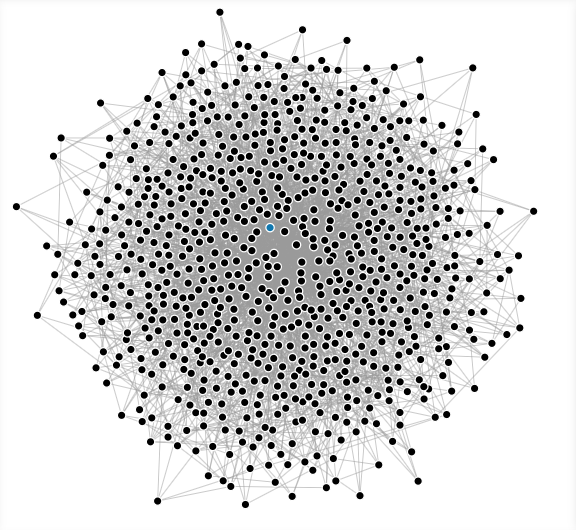
\includegraphics[width=1\linewidth]{figs/barabasi-albert-0}
\caption{$T=0$}
\end{subfigure}%
\begin{subfigure}[b]{.5\linewidth}
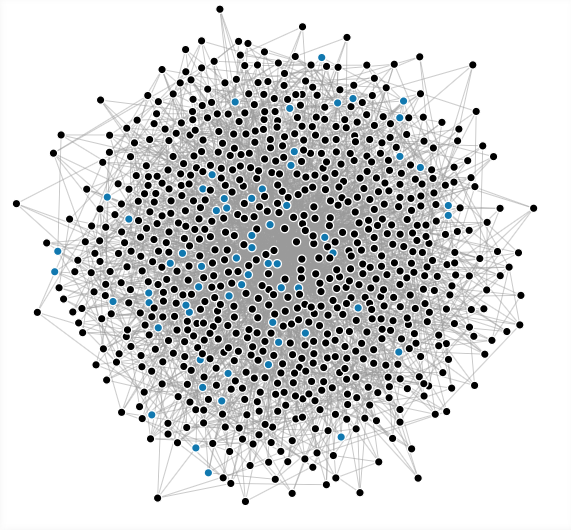
\includegraphics[width=1\linewidth]{figs/barabasi-albert-4}
\caption{$T=4$}
\end{subfigure}

\begin{subfigure}[b]{.5\linewidth}
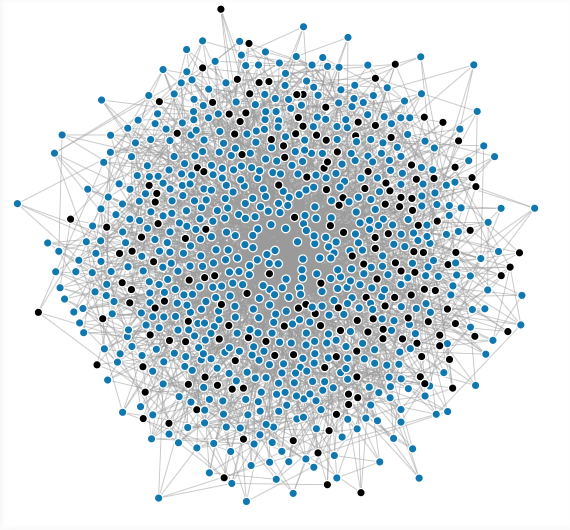
\includegraphics[width=1\linewidth]{figs/barabasi-albert-8}
\caption{$T=8$}
\end{subfigure}%
\begin{subfigure}[b]{.5\linewidth}
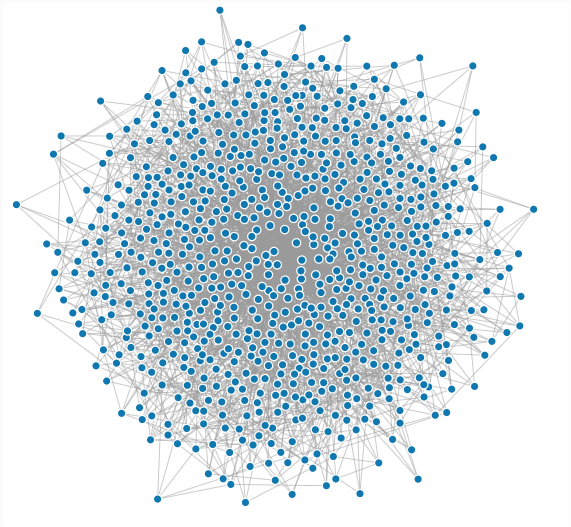
\includegraphics[width=1\linewidth]{figs/barabasi-albert-12}
\caption{$T=12$}
\end{subfigure}

\caption{Rumor spreading (blue nodes) in Barabasi Albert graph with $n=800$, $m_0 = 20$ and $M = 4$}
\label{barabasi-albert-graphs}
\end{figure}

\begin{figure}
\centering
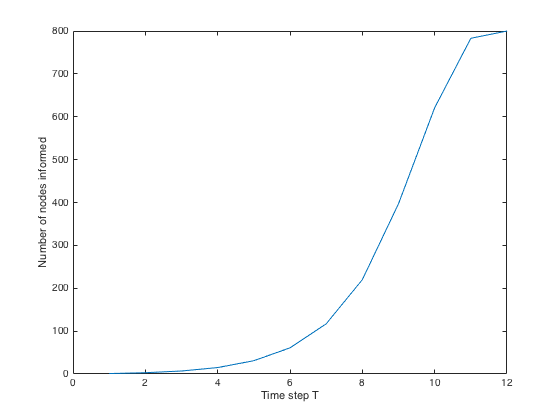
\includegraphics[width=1\linewidth]{figs/barabasi-albert-chart}
\caption{Number of nodes informed over time in the Barabasi Albert simulation}
\label{fig:barabasi-albert-chart}
\end{figure}

Intuitively it would be much more interesting to study more malformed graphs where some nodes are hard to reach. We will start with a simple example of a graph composed of two distinct graphs $C(n,p)$ with very few connections between the two. Those edges will form a bottle neck harder to cross for the gossip. Given that this bottle neck is a very good cut, this graph will have a very low conductance and the constant in the $\log n$ would be affected badly. The edges between the two distinct populations are picked independently and uniformly with probability $q$ in our simulation.

\begin{figure}
\centering

\begin{subfigure}[b]{.5\linewidth}
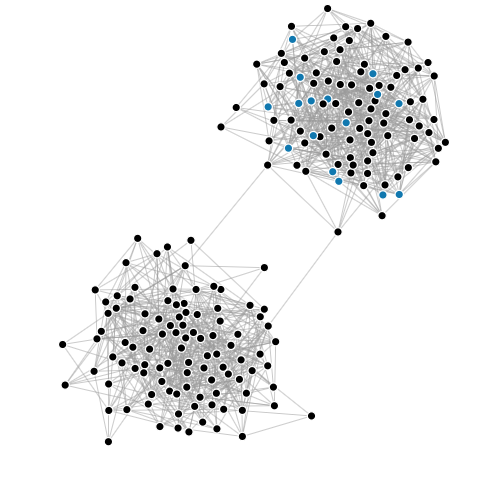
\includegraphics[width=1\linewidth]{figs/split-1}
\caption{$T=3$}
\end{subfigure}%
\begin{subfigure}[b]{.5\linewidth}
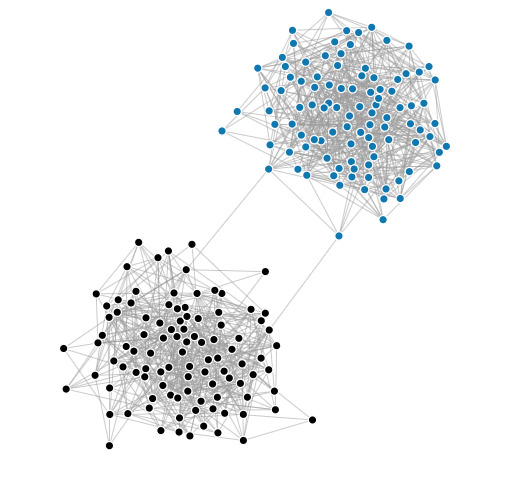
\includegraphics[width=1\linewidth]{figs/split-2}
\caption{$T=7$}
\end{subfigure}

\begin{subfigure}[b]{.5\linewidth}
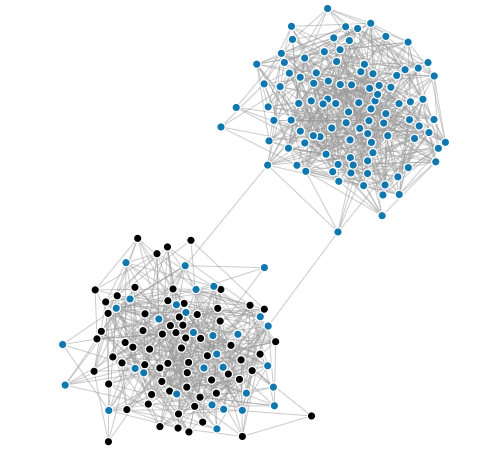
\includegraphics[width=1\linewidth]{figs/split-3}
\caption{$T=12$}
\end{subfigure}%
\begin{subfigure}[b]{.5\linewidth}
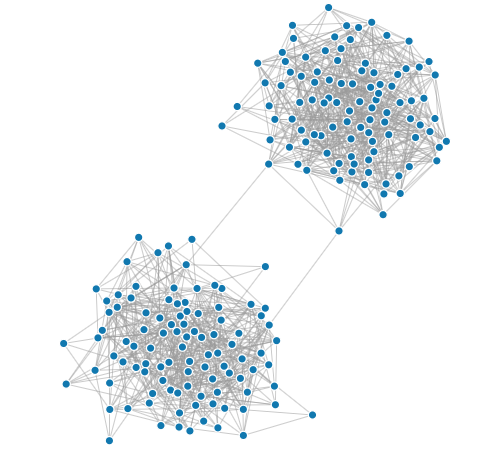
\includegraphics[width=1\linewidth]{figs/split-4}
\caption{$T=15$}
\end{subfigure}

\caption{Rumor spreading (blue nodes) in bottleneck model with $n=85$, $p = 0.1$ and $q = 0.0003$}
\label{barabasi-albert-graphs}
\end{figure}


\begin{figure}
\centering
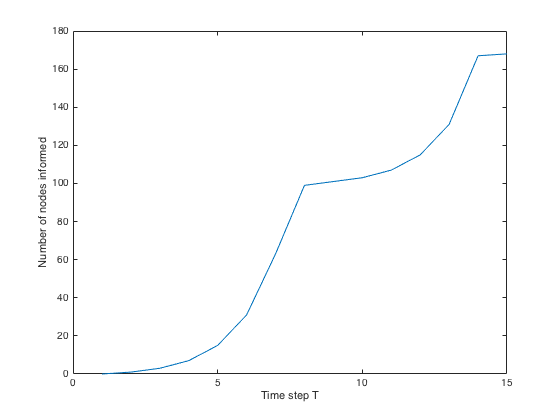
\includegraphics[width=1\linewidth]{figs/split-chart}
\caption{Number of nodes informed over time in the bottleneck simulation}
\label{fig:split-chart}
\end{figure}

We can see in \cref{fig:split-chart} that the number of informed nodes palliates when the rumor has to cross the bottleneck. It is normal that the topology of a network affects the quality of the broadcast and bridging an information between two very well distinct populations is hard.

\begin{thebibliography}{1}

\bibitem{guosun}
Z.~Guo, H.~Sun, 
\emph{Gossip vs. Markov Chains, and Randomness-Efficient Rumor Spreading}.\hskip 1em plus
0.5em minus 0.4em\relax Proceedings of the Twenty-Sixth Annual ACM-SIAM Symposium on Discrete Algorithms, SODA 2015, San Diego, CA, USA, January 4-6, 2015.

\bibitem{jerrum}
M.~Jerrum, A.~Sinclair, 
\emph{Conductance and the rapid mixing property for Markov chains: the approximation of permanent resolved}.\hskip 1em plus
0.5em minus 0.4em\relax Proceedings of the twentieth annual ACM symposium on Theory of computing.

\bibitem{coupling}
T.~Lindvall, 
\emph{Lectures on the Coupling Method}.\hskip 1em plus
0.5em minus 0.4em\relax New York, 2002.

\end{thebibliography}

\end{document}


